\section{ML Workload Optimizations} \label{sec-ml-workloads}
In this section, we first describe the common types of operations in machine learning workloads.
Then, we discuss how to capture and store the operations in the experiment graph.
Lastly, we discuss how do we utilize the experiment graph to optimize new workloads.

\subsection{Operations in ML Workloads}
We assume the main units of work are data frame (e.g., Pandas, R Data Frames, and Spark Data Frames) like objects that contain one or many columns, where all the data items in one column are of the same data type.
\hl{We divide the operations in the ML workloads into 3 categories.}
% Tilmann: Are these balanced? It seems to me that Hyper parameter training is part of the model training. Behrouz: The point I'm trying to make is that hyperparameter tuning are repeated model training operations. So technically, when there are opportunities for reuse and warmstarting inside hyperparameter tuning, our optimizer will use them. But, there are still two other opportunities that are specific to hyperparameter tuning. 1) Hyperparameter tuning require search space definition, using the experiment graph, we can automatically define the space 2) Bayesian/Sequential hyperparameter tuning requires past knowledge in form of many initial model training to perform better, using the experiment graph we can provide this 'past knowledge' without actually executing the initial model training.
\begin{table}
\centering
\begin{tabular}{ll}
\hline
	   Feature Extraction & Feature Selection\\ \hline
        feature hasher & variance threshold  \\
        one hot encoding & select k best \\
        count vectorizer& select percentile \\ 
        tfidf transformer & recursive feature elimination \\
        hashing vectorizer & select from model \\
        extract\_patch\_2d &  \\
        \hline
\end{tabular}
\caption{List of feature extraction and feature selection operations}\label{feature-engineering-operations}
\end{table}

\subsubsection{Data and Feature Engineering}
This group of operations typically belongs to three categories, i.e., simple data transformations and aggregations, feature selection, and feature extraction.
All of these operations, receive one or multiple columns of a dataset and return another dataset as result. 
While different data processing tools may provide specialized data transformation and aggregation operations for data frame objects, most of them provide the same or similar operations such as map, reduce, group by, concatenation, and join. 
In Table \ref{feature-engineering-operations}, we show a list of the most common feature extraction and feature selection operations.

\subsubsection{Model Training}
Model training operations are a group of operations that receive a dataset and return a machine learning model.
The result of model training operations can either be used in other data and feature engineering operations (e.g., applying PCA to reduce the number of dimensions of the data) or can be used to perform prediction (for classification and regression tasks) on unseen data.

\subsubsection{Hyperparameter Tuning}
Before training a machine learning model, one has to set the hyperparameters of the model to appropriate values.
Typically, the best values for the hyperparameters of a model vary across different datasets.
The goal of hyperparameter tuning operations is to find the set of hyperparameters that yield the model with the best performance on a dataset.
A hyperparameter tuning operation is defined by a budget, a search method, and a search space.
The budget specifies how many models with different hyperparameter values, within the specified search space, should be trained and the search method specifies what search strategy to incorporate.
The most common search methods are grid search, random search, and Bayesian hyperparameter search \cite{bergstra2012random,snoek2012practical}.

\subsection{Experiment Graph Representation}\label{sub-graph-construction}
We represent a collection of machine learning workloads as the graph $G(V, E)$ which we refer to as the experiment graph.
$V=\{v_i\}, i = 1, \cdots, n$ is the set of all the artifacts in the workloads.
Each artifact is either a raw dataset, a pre-processed dataset resulting from a feature engineering operation, or a model resulting from a model training operation.
$E=\{e_i\}, i = 1, \cdots, m$ is the set of all the executed operations in the workloads.
A directed edge $e$ from $v_i$ to $v_j$ in $G(V, E)$ indicates that the artifact $v_j$ is derived from the artifact $v_i$ by applying the operation in $e$.
Every vertex $v$ has the attributes $\langle f, s \rangle$ (accessed by $v.f$ and $v.s$), which represent the  frequency, i.e., number of different workloads an artifact appears in, and storage size of artifact.
Every edge $e$ has the attribute $\langle t \rangle$ (accessed by $e.t$), which represent the run-time (in seconds) of the operation.

%TODO I'm still not sure if we need to have edge frequency as well (number of times an operation is executed). In the current version of the materialization algorithms, we are only using vertex frequency. I ll keep this todo here for now, just in case we may realize edge frequency is also important. 
%In many cases, the vertex access frequency is equal to the execution frequency of its incoming edge.
%However, we make the distinction between the two in cases where users explicitly access the content of the vertex, either by printing them or saving them to disk.

Each vertex contains the data (inside the data frame) and meta-data of the artifacts, such as the name and type of the columns for datasets and name, size, the value of parameters and hyperparameters, and the error metric of the models.
Each edge contains the meta-data of the operation, such as the function name, training algorithm, hyperparameters, and in some cases even the source code of the operation.
When a new machine learning workload is executed, we update the experiment graph by adding the new artifacts and operations.
If any of the artifacts already exist in the graph, their frequency is updated.

Figure \ref{fig-experiment-graph}a shows an example graph constructed from the code in Listing \ref{listing-experiment-graph}.
To uniquely identify an edge, we utilize a hash function that receives as input the operation and its hyperparameters (if it has any).

\begin{lstlisting}[language=Python, caption=Example script,captionpos=b,label = {listing-experiment-graph}]
import numpy as np
import pandas as pd

from sklearn import svm
from sklearn.feature_selection import SelectKBest
from sklearn.feature_extraction.text import CountVectorizer

train = pd.read_csv('../input/train.csv') 
print train.columns # [ad_desc,ts,u_id,price,y]
vectorizer = CountVectorizer()
count_vectorized = vectorizer.fit_transform(train['ad_desc'])
selector =  SelectKBest(k=2)
top_features = selector.fit_transform(train[['ts','u_id','price']], 
				      train['y'])
top_features # print the content of the data frame			     
X = pd.concat([count_vectorized,top_features], axis = 1)
model = svm.SVC().fit(X, train['y'])
\end{lstlisting}

\begin{figure}
\begin{subfigure}[b]{0.4\linewidth}
\centering
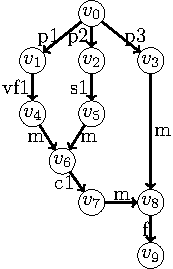
\includegraphics[width=0.8\linewidth]{../images/tikz-standalone/example-graph}
\caption{}
\end{subfigure}%
\begin{subfigure}[b]{0.6\linewidth}
\begin{tabular}{lcl}
\hline
operation & label &  hash \\
\hline
project(ad..) & $\langle 2s\rangle$ &p1 \\
project(ts, ..) & $\langle 6s\rangle$ & p2\\
project(y) & $\langle 2s\rangle$ & p3\\
vectorizer.f\_t & $\langle 40s\rangle$ & vf1 \\
selector.f\_t & $\langle 60s\rangle$ & s1 \\
concat & $\langle 10s\rangle$ & c1 \\
merge & $\langle 0s\rangle$ & m\\
svm.fit & $\langle 100s\rangle$ & f\\
\hline
\end{tabular}
\caption{}
\end{subfigure}
\caption{Experiment graph constructed from the Listing \ref{listing-experiment-graph} (a) and the hash of the operations in the scripts (b)}
\label{fig-experiment-graph}
\end{figure}
Table \ref{fig-experiment-graph}b shows both the label of every edge operation, i.e., time, and the hash of the operations and their hyperparameters.
Since at the time of the execution of the script, the experiment graph is empty, all the artifacts (vertices) have a frequency of 1.
In order to represent operations that process multiple input artifacts, e.g., concat and svm.fit operations in Listing \ref{listing-experiment-graph}, we proceed as follows.
First, we merge the vertices representing the artifacts into a single vertex using a merge operator.
The merge operator is a logical operator which does not incur a cost, i.e., it has a run-time of 0 seconds.
The merged vertex is also a logical vertex with no actual attributes which only contains the vertex id of the merged vertices.
Then, we draw an edge from the merged vertex which represents the actual operation.
For example, in Figure \ref{fig-experiment-graph}a, before applying the concatenation operation, we merge $v_4$ and $v_5$ into $v_6$, then we apply the concatenation operation (c1).
%TODO Do I need to explain why we're doing this? 
%This is a critical step for the materialization algorithms and optimization strategies.

\subsection{Workload Optimizer for Kaggle Use Case}
By utilizing an experiment graph, we design a workload optimizer framework.
We integrate the workload optimizer into collaborative data science platform to improve the execution of the workloads.
Here, we describe the integration process of the workload optimizer for optimizing and executing kernels in the Kaggle use case (our motivating example).

Figure \ref{improved-use-case} shows the process of the workload optimization in the Kaggle Infrastructure. 
The workflow is as follows.
First, we parse a workload (i.e., a kernel) and construct the workload graph (\circledtext{1}).
Then, an \textbf{optimizer} component receives the workload graph and utilizes the existing experiment graph to look for optimization opportunities, namely, reusing the existing operations, warmstarting the model training, and for workloads that contain a hyperparameter tuning operation, faster hyperparameter search (\circledtext{2}).
The result of the optimization is another workload graph which contains precomputed artifacts, warmstarted models, and proper search space and/or an initialized Bayesian hyperparameter search process.
After executing the optimized workload, we return the result to the user (\circledtext{3}).
After the execution, we update the experiment graph using the original workload graph (\circledtext{4}).
Finally, to ensure that we can store the experiment graph given our storage budget, we run our materialization algorithms to decide what artifacts to materialize (\circledtext{5}).

\begin{figure}
\centering
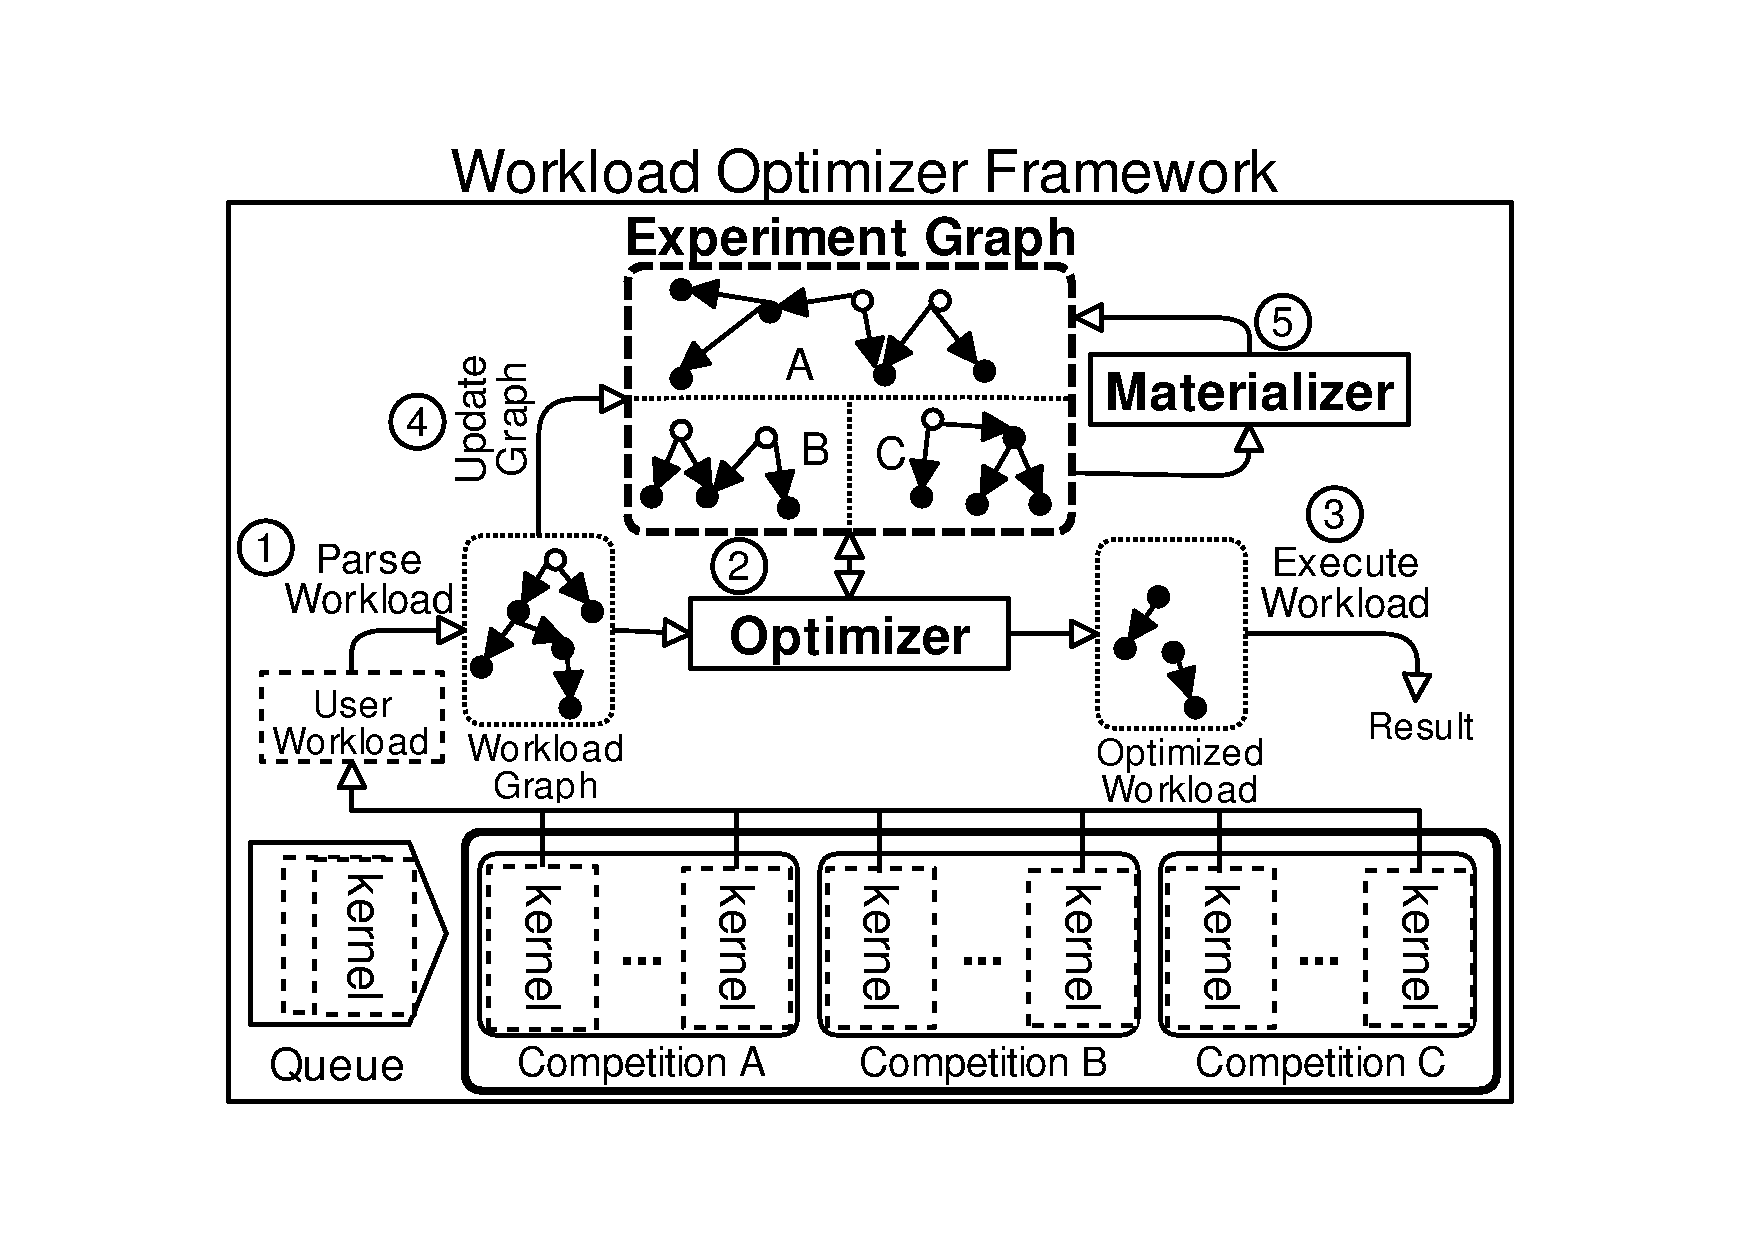
\includegraphics[width=\columnwidth]{../images/kaggle-workload-optimizer}
\caption{Improving the execution of Kaggle Kernels with Workload Optimizer}
\label{improved-use-case}
\end{figure}

It is important to note that we restrict the scope of our optimizations and materialization algorithms to one machine learning task. 
In Kaggle, each competition defines the machine learning task, i.e., one or multiple raw training datasets (we refer to as root datasets), a validation data set, and an evaluation function which computes the quality/error rate of the model on the validation dataset.
While the experiment graph contains artifacts from all the competitions (tasks), each task corresponds to a unique connected component in the experiment graph.
When optimizing a new workload, we only utilize the relevant connected component.
In Figure \ref{improved-use-case}, the experiment graph has three connected components representing the three competitions, A, B, and C which are rooted at 2, 2, and 1 root training datasets, depicted as hollow vertices, respectively.
When optimizing a new Kaggle kernel from competition A, we only look for optimization opportunities in the connected component A of the experiment graph.